\include{Macros/MacroFile1}
\documentclass[oneside,11pt]{Classes/myThesis}
%%%%%%%%%%%%%%%%%%%%%%%%%%%%%%%%%%%%%%%%%%%%%%%%%%%%%%
%%%%%%%%%%%%%%%%%%% Instructions %%%%%%%%%%%%%%%%%%%%%
%%%%%%%%%%%%%%%%%%%%%%%%%%%%%%%%%%%%%%%%%%%%%%%%%%%%%%
%% Fill in the details about your name, and project title
%% in the sections just below here. Then you write each
%% Chapter in a separate LaTeX file - you will find Chapter 1
%% is already setup for you.
%%
%% The folder structure is:
%% Chapters
%%     |-----------> Chapter_1
%%     |                  |----------> Chapter_1_Fig
%%     |                  |               |-> My_fig.eps
%%     |                  |----------> Chapter_1_file.tex
%%     !-----------> Chapter_2
%%     |                  |----------> Chapter_2_Fig
%%     |                  |               |-> My_other_fig.eps
%%     |                  |----------> Chapter_2_file.tex
%%
%% Chapter_1 contains an exa,ple of includinga figure in the text with a reference.
%%%%%%%%%%%%%%%%%%%%%%%%%%%%%%%%%%%%%%%%%%%%%%%%%%%%%%
%%%%%%%%%%%%%%% file path for figures - add extra chapters as necessary %%%%%%%%%
%%%%%%%%%%%%%%%%%%%%%%%%%%%%%%%%%%%%%%%%%%%%%%%%%%%%%%
\graphicspath{{./Chapters/Chapter_1/Chapter_1_Fig/}     
              {./Chapters/Chapter_2/Chapter_2_Fig/}
              {./Chapters/Chapter_3/Chapter_3_Fig/}
              {./ThesisFigs/}}

%%%%%%%%%%%%%%%%%%%%%%%%%%%%%%%%%%%%%%%%%%%%%%%%%%%%%%
%%%%%%%%%%%%% Constants - fill these in for use throughout the thesis %%%%%%%%%%%%
%%%%%%%%%%%%%%%%%%%%%%%%%%%%%%%%%%%%%%%%%%%%%%%%%%%%%%
\newcommand{\theAuthor}{Your Full name}
\newcommand{\authorEmail}{physpqr@leeds.ac.uk}
\newcommand{\myTitle}{My Project  Title}
\newcommand{\supervisor}{Prof. M.Y. Supervisor}
%%%%%%%%%%%%%%%%%%%%%%%%%%%%%%%%%%%%%%%%%%%%%%%%%%%%%%
\pdfinfo { /Title  (\myTitle)
           /Creator (TeX)
           /Producer (pdfTeX)
           /Author (\theAuthor \authorEmail)
           /ModDate (D:\pdfdate)
           /CreationDate (D:\pdfdate)  %format D:YYYYMMDDhhmmss
           /Subject (Condensed Matter Physics)
           /Keywords (BSc, Report)}    
		\pdfcatalog { /PageMode (/UseOutlines)
                  /OpenAction (fitbh)  }

%%%%%%%%%%%%%%%%%%%%%%%%%%%%%%%%%%%%%%%%%%%%%%%%%%%%%%
%%%%%%%%%%%%% Title Page Information %%%%%%%%%%%%%%%%%%%%%%%%%%%%
%%%%%%%%%%%%%%%%%%%%%%%%%%%%%%%%%%%%%%%%%%%%%%%%%%%%%%
\title{\myTitle}
\author{\href{mailto:\authorEmail}{\theAuthor}}
\crest{\includegraphics[width=35mm]{Leeds_Crest.png}}
%%%%%%%%%%%%%%%%%%%%%%%%%%%%%%%%%%%%%%%%%%%%%%%%%%%%%%
%% Define these as empty to omit the two logos on the title page
%%%%%%%%%%%%%%%%%%%%%%%%%%%%%%%%%%%%%%%%%%%%%%%%%%%%%%
\logo{\includegraphics[width=50mm]{UoL_logo}} %University Logo
\deptlogo{} %\includegraphics[width=50mm]{UoL_logo}} % Institute Logo
%%%%%%%%%%%%%%%%%%%%%%%%%%%%%%%%%%%%%%%%%%%%%%%%%%%%%%
\collegeordept{\href{http://physics.leeds.ac.uk}{School of Physics and Astronomy}}
\university{\href{http://www.leeds.ac.uk}{University of Leeds}}

\degree{Bachelor of Science}
\degreedate{\monthdate\today}

%Different font in captions
%Different font in caption
%%%%%%%%%%%%%%%%%%%%%%%%%%%%%%%%%%%%%%%%%%%%%%%%%%%%%%
%%%%%%%%%%%%%%%% Optional Packages  %%%%%%%%%%%%%%%%%%%%%%%%%%%
%%%%%%%%%%%%%%%%%%%%%%%%%%%%%%%%%%%%%%%%%%%%%%%%%%%%%%
%\usepackage{StyleFiles/watermark}
%\usepackage{xspace}  %add a space after maths if not already there
%\usepackage{booktabs} %better tables
%\usepackage{rotating}  %rotating figures and tables
% \usepackage{array} %enhanced tables
%\usepackage{ctable} %include a figure command
%\usepackage{footnote}
%\usepackage{multirow} %for merging cells on tables
%\usepackage{times} % The "Times" font
%\usepackage{Utopia} % The "Utopia" font

\linespread{1.3} %1.5 line spacing

\begin{document}
%\baselineskip=18pt plus1pt

\maketitle
%set the number of sectioning levels that get number and appear in the contents
\setcounter{secnumdepth}{2}
\setcounter{tocdepth}{2}
\pagenumbering{roman}
\frontmatter
%%%%%%%%%%%%%%%%%%%%%%%%%%%%%%%%%%%%%%%%%%%%%%%%%%%%%%
%%%%%%%%%%%% Include sections are required, or comment out to skip over %%%%%%%%%
%%%%%%%%%%%%%%%%%%%%%%%%%%%%%%%%%%%%%%%%%%%%%%%%%%%%%%
%\include{Dedication/dedication}
\include{IPStatement/ipstatement}
\include{Acknowledgement/acknowledgement}
\include{Abstract/abstract}
\newpage
\tableofcontents
\newpage
\listoffigures
\newpage
\listoftables
\newpage
\include{Abbreviations/Abbreviations}
%\include{Common_Symbols/Common_Symbols}

\mainmatter

\pagenumbering{arabic}
\chapter{Introduction}
Thesis writing is lots of fun.

Lorem ipsum dolor sit amet, consectetur adipiscing elit, sed do eiusmod tempor incididunt ut labore et dolore magna aliqua. Ac turpis egestas maecenas pharetra. Ultrices dui sapien eget mi proin sed libero. Pretium vulputate sapien nec sagittis aliquam malesuada. Turpis egestas maecenas pharetra convallis. Sed risus ultricies tristique nulla. Vulputate enim nulla aliquet porttitor lacus luctus accumsan tortor posuere. Mi sit amet mauris commodo quis. Purus semper eget duis at tellus at urna. Sit amet purus gravida quis blandit. Eleifend quam adipiscing vitae proin sagittis nisl rhoncus. At imperdiet dui accumsan sit amet nulla facilisi morbi. In arcu cursus euismod quis viverra. Sed adipiscing diam donec adipiscing. Euismod lacinia at quis risus sed vulputate odio ut enim. Nulla malesuada pellentesque elit eget gravida. Proin libero nunc consequat interdum varius sit amet mattis vulputate. Donec enim diam vulputate ut pharetra sit.

Varius morbi enim nunc faucibus. Eget duis at tellus at urna condimentum. Aliquam id diam maecenas ultricies mi eget. Eget velit aliquet sagittis id consectetur purus ut faucibus pulvinar. In vitae turpis massa sed elementum tempus egestas. Massa placerat duis ultricies lacus. Ut etiam sit amet nisl purus in mollis nunc sed. Faucibus vitae aliquet nec ullamcorper sit amet risus nullam. Aenean sed adipiscing diam donec. Volutpat sed cras ornare arcu.

Sed augue lacus viverra vitae congue eu consequat ac felis. Viverra adipiscing at in tellus integer. Sed pulvinar proin gravida hendrerit. Non tellus orci ac auctor augue. Suspendisse sed nisi lacus sed viverra tellus. Cum sociis natoque penatibus et. Nibh tortor id aliquet lectus. Egestas erat imperdiet sed euismod nisi. Magnis dis parturient montes nascetur ridiculus. Sit amet mattis vulputate enim nulla aliquet porttitor. Enim ut tellus elementum sagittis vitae et. Amet commodo nulla facilisi nullam vehicula ipsum. Viverra vitae congue eu consequat ac felis. Mattis enim ut tellus elementum sagittis vitae et. Velit laoreet id donec ultrices tincidunt arcu. Amet facilisis magna etiam tempor orci. Eu tincidunt tortor aliquam nulla facilisi cras fermentum odio. Eu scelerisque felis imperdiet proin.

Etiam tempor orci eu lobortis elementum nibh tellus. Mattis enim ut tellus elementum sagittis vitae et. Cras adipiscing enim eu turpis egestas pretium aenean pharetra. Risus sed vulputate odio ut. At auctor urna nunc id cursus metus aliquam eleifend mi. Facilisi morbi tempus iaculis urna id volutpat. Cras adipiscing enim eu turpis egestas. Volutpat blandit aliquam etiam erat velit scelerisque in. Eu nisl nunc mi ipsum faucibus vitae aliquet nec ullamcorper. Tortor aliquam nulla facilisi cras fermentum odio. Commodo sed egestas egestas fringilla. Vulputate ut pharetra sit amet aliquam id. Ac tortor dignissim convallis aenean et tortor at risus viverra. Ridiculus mus mauris vitae ultricies leo integer. Suscipit adipiscing bibendum est ultricies integer quis auctor elit sed.

\begin{figure}
	\centering
	\includegraphics[width=0.5\linewidth]{slimshady_new}
	\caption{An example of how to place a figure with a caption and a lebel that you can use to cross reference the figure. Don't forget to cist the source of copied figures \cite{Batley2015} and put the label after the caption to make the cross referenced figure number correct.}
	\label{fig:fig_label}
\end{figure}

Always make sure that every figure is referred to in the text. Here, for example, figure \ref{fig:fig_label} shows one of our instruments. Tables work just like figurwes - see table \ref{tab:table_ex} for example

Non quam lacus suspendisse faucibus interdum posuere lorem ipsum dolor. Eu nisl nunc mi ipsum faucibus. Justo eget magna fermentum iaculis eu. Lacus suspendisse faucibus interdum posuere lorem. Fusce ut placerat orci nulla pellentesque dignissim enim. Vitae proin sagittis nisl rhoncus mattis rhoncus. Commodo nulla facilisi nullam vehicula ipsum. Nunc sed velit dignissim sodales ut eu. Elit pellentesque habitant morbi tristique senectus et netus et malesuada. Enim sit amet venenatis urna cursus. Phasellus vestibulum lorem sed risus ultricies. Magna eget est lorem ipsum dolor. Nulla aliquet porttitor lacus luctus accumsan. Vitae et leo duis ut. Nec tincidunt praesent semper feugiat nibh sed pulvinar proin gravida. Phasellus faucibus scelerisque eleifend donec pretium vulputate sapien nec. Amet risus nullam eget felis eget. Sodales ut etiam sit amet. Nisl condimentum id venenatis a. Neque viverra justo nec ultrices dui.

Vitae aliquet nec ullamcorper sit amet risus nullam eget felis. Egestas egestas fringilla phasellus faucibus scelerisque eleifend donec pretium. In est ante in nibh mauris cursus. Cursus in hac habitasse platea dictumst quisque sagittis. Orci ac auctor augue mauris augue neque gravida. Nullam ac tortor vitae purus faucibus ornare suspendisse. Diam donec adipiscing tristique risus nec feugiat in. Leo vel fringilla est ullamcorper eget nulla facilisi etiam. Eu augue ut lectus arcu bibendum at. In fermentum posuere urna nec tincidunt praesent. Ornare quam viverra orci sagittis eu volutpat odio. Pellentesque habitant morbi tristique senectus et.

\begin{table}
	\begin{center}
\begin{tabular}{ |p{3cm}||p{3cm}|p{3cm}|p{3cm}|  }
	\hline
	\multicolumn{4}{|c|}{Country List} \\
	\hline
	Country Name     or Area Name& ISO ALPHA 2 Code &ISO ALPHA 3 Code&ISO numeric Code\\
	\hline
	Afghanistan   & AF    &AFG&   004\\
	Aland Islands&   AX  & ALA   &248\\
	Albania &AL & ALB&  008\\
	Algeria    &DZ & DZA&  012\\
	American Samoa&   AS  & ASM&016\\
	Andorra& AD  & AND   &020\\
	Angola& AO  & AGO&024\\
	\hline
\end{tabular}
\caption{Tables are always a git of a pain in \LaTeXe - but here is an example table taken from \url{https://www.overleaf.com/}. Make sure the label goes after the caption for figures and tables!}
\label{tab:table_ex}
\end{center}	
\end{table}

Lorem ipsum dolor sit amet. Ipsum dolor sit amet consectetur adipiscing elit. Tortor vitae purus faucibus ornare suspendisse sed nisi lacus. Quis enim lobortis scelerisque fermentum dui faucibus in ornare quam. Turpis egestas sed tempus urna. Id nibh tortor id aliquet. Sed tempus urna et pharetra pharetra massa. Sit amet mauris commodo quis imperdiet. Sed felis eget velit aliquet sagittis id. Id diam maecenas ultricies mi eget mauris. Aliquet nec ullamcorper sit amet risus nullam eget felis. Nascetur ridiculus mus mauris vitae. Ultrices vitae auctor eu augue ut lectus. Dolor sed viverra ipsum nunc aliquet. Consequat ac felis donec et odio pellentesque diam volutpat commodo. Fermentum dui faucibus in ornare. Blandit massa enim nec dui nunc mattis. Dictum varius duis at consectetur lorem donec massa sapien. Sed arcu non odio euismod lacinia at quis.

\begin{figure}
	\centering
	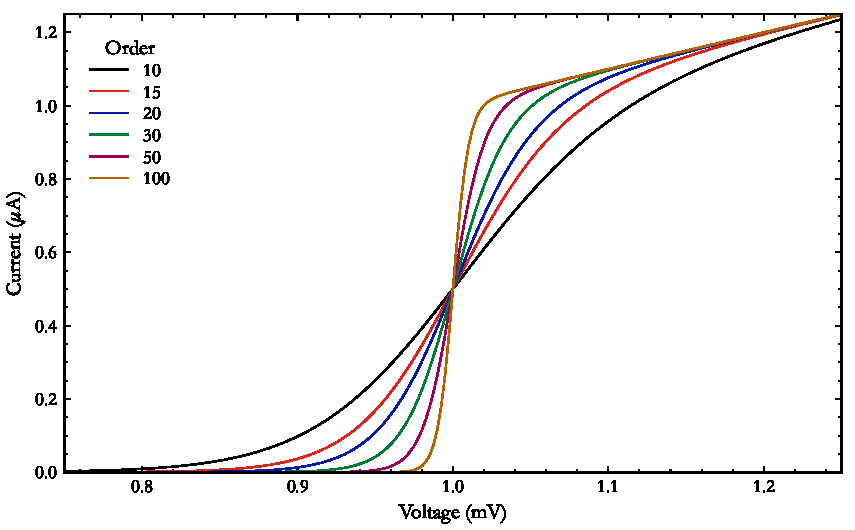
\includegraphics{fig02h_0}
	\caption{If you are making figures with Python, then I strongly recommend that you
		use the \textbf{stonerplots}\cite{stonerplots} package. It has a ``thesis'' style that is set up
		for this template.}
	\label{fig:fig_label}
\end{figure}

\begin{figure}
	\centering
	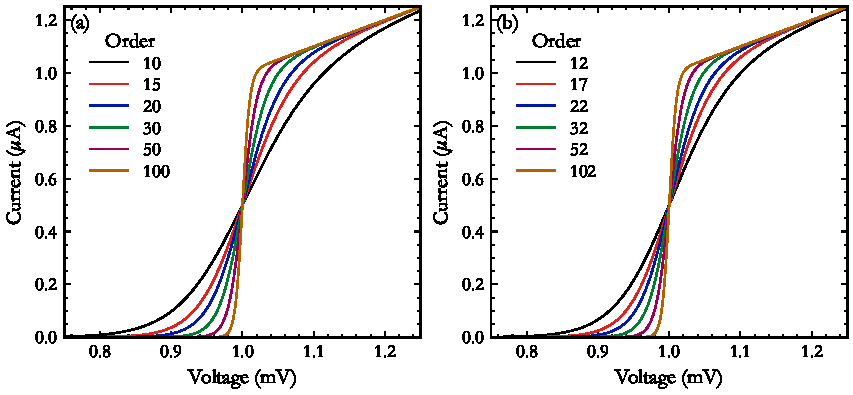
\includegraphics{fig02h_1}
	\caption{Double panel figures are also easily made with the \textbf{stonerplots}\cite{stonerplots} packae.
	and the MultiPanel context manager.}
	\label{fig:fig_label}
\end{figure}



Aliquam vestibulum morbi blandit cursus risus at ultrices. Euismod nisi porta lorem mollis aliquam ut. Pellentesque nec nam aliquam sem et tortor. Nunc sed augue lacus viverra vitae congue eu consequat ac. Feugiat nisl pretium fusce id velit ut. Dolor magna eget est lorem ipsum dolor sit. Faucibus ornare suspendisse sed nisi lacus sed viverra tellus. In nulla posuere sollicitudin aliquam. Habitant morbi tristique senectus et netus et malesuada. Tempor id eu nisl nunc mi ipsum faucibus vitae. Posuere morbi leo urna molestie at elementum. Euismod quis viverra nibh cras pulvinar mattis. Egestas pretium aenean pharetra magna ac placerat. Sit amet volutpat consequat mauris nunc congue nisi vitae suscipit. Vel pharetra vel turpis nunc eget lorem dolor. Id consectetur purus ut faucibus pulvinar elementum.


Volutpat maecenas volutpat blandit aliquam etiam. Magna fringilla urna porttitor rhoncus dolor purus non enim praesent. Ornare quam viverra orci sagittis. Consequat id porta nibh venenatis cras sed felis eget velit. Amet consectetur adipiscing elit ut aliquam purus sit. Ultrices tincidunt arcu non sodales neque. Vitae congue mauris rhoncus aenean vel elit scelerisque. Nunc faucibus a pellentesque sit amet porttitor. Faucibus vitae aliquet nec ullamcorper sit amet risus. Fringilla urna porttitor rhoncus dolor purus non enim praesent. Diam maecenas ultricies mi eget mauris. Amet aliquam id diam maecenas ultricies. Massa enim nec dui nunc. Tempor nec feugiat nisl pretium fusce. Risus nullam eget felis eget nunc. Sed odio morbi quis commodo odio. Porttitor massa id neque aliquam vestibulum morbi blandit cursus. Vitae tempus quam pellentesque nec nam aliquam sem.

At ultrices mi tempus imperdiet nulla malesuada. Cum sociis natoque penatibus et magnis. Mattis pellentesque id nibh tortor id aliquet lectus proin nibh. Facilisis volutpat est velit egestas dui id ornare arcu. Cras ornare arcu dui vivamus arcu felis bibendum. Senectus et netus et malesuada. Nunc mattis enim ut tellus. Eu mi bibendum neque egestas congue quisque egestas diam in. Mattis nunc sed blandit libero. A cras semper auctor neque vitae tempus. Porttitor eget dolor morbi non arcu. Magna ac placerat vestibulum lectus mauris ultrices. Vulputate sapien nec sagittis aliquam malesuada bibendum. %% file path for chapter tex files 
\include{Chapters/Chapter_2/Chapter_2_File}
%\include{Chapters/Chapter_3/Chapter_3_File}
%\include{Chapters/Chapter_4/Chapter_4_File}
%\include{Chapters/Chapter_5/Chapter_5_File}
%\include{Chapters/Chapter_6/Chapter_6_File}


\appendix
\chapter{Material not in a chapter}
This is the first appendix.

\section{Bits of \LaTeX advice}

\begin{enumerate}
	\item Do look at the output log and try to understand any errors - they are sometimes important!
	\item In the final pdf, do a search for ? - it is what \LaTeX will give when a reference is missing. Having missing references in your submitted thesis is, at best, embarrassing and potentially a failing matter.
	\item A good quality bib file is important - make sure that entries are consistent in whether journals are abreviated, capitalised and how Author names are presented. A good way to do this is to use Mendeley to import your bib file and then use its doi lookup feature which will re-write your bibliogrpahy entries in a standardised form. You then export the bibliography back oit as a bib file.
	\item Be particularly careful about older papers where the doi may not be easy to track down. Also watch out for JETP Letters that you are being consistent in citing the English language version (or the Russian, but don't mix and match!)
	\item Although \LaTeX guides may show you how to assemble a multi-part fgure from within \LaTeX, it can be hard to make sub-plots appear exactly the same size. We recommend using something like Inkscape to assemble the parts of a figure and lay them out nicely. Be careful if saving to pdf files thatr the fonts are preserved - otherwise you can lose greek symbols.
	\item If preparing figures in Origin, set the plot size to be exactly the right size or exactly double size and then scale fonts and symbols accordingly. Use Origin's ability to copy formatting between graphs to make everything nicely consistent (e.g. frame sizes, thicknesses, coolour schemes, point sizes and shapes).
	\item In general resist the temptation to put [H] when placing figures and tables - in most cases it is better to let \LaTeX work out where to put things. It can get tricky if you have a lot of figures one after another (perhaps a single multi-part figure is what you need?) - the placement option [p] can alos help to move floats to a separate page of figures. See also the \textit{afterpage} package. 
\end{enumerate}
%\include{Appendix2/Appendix2}
%. More appendicies here.
\addcontentsline{toc}{chapter}{References} % Adds References to contents page
\bibliographystyle{ieeetr_me} % bibliography style
\renewcommand{\bibname}{References} 
\bibliography{References/library} % References file
\end{document}